\documentclass[a4paper, 12pt]{article}%тип документа

%отступы
\usepackage[left=1.5cm,right=1cm,top=2cm,bottom=3cm,bindingoffset=0cm]{geometry}
\setlength{\parindent}{5ex}

%Русский язык
\usepackage[T2A]{fontenc} %кодировка
\usepackage[utf8]{inputenc} %кодировка исходного кода
\usepackage[english,russian]{babel} %локализация и переносы

%Вставка картинок
\usepackage{graphicx}
\graphicspath{{pictures/}}
\DeclareGraphicsExtensions{.pdf,.png,.jpg,}
\usepackage{wrapfig}

%Графики
\usepackage{pgfplots}
\pgfplotsset{compat=1.9}

%Математика
\usepackage{amsmath, amsfonts, amssymb, amsthm, mathtools}
\usepackage{derivative}

%Таблицы
\usepackage{longtable} 
\usepackage{float}

%Римские цифры
\newcommand{\RomanNumeralCaps}[1]{\uppercase\expandafter{\romannumeral#1}}

\usepackage{multirow}

\usepackage{listings}
\lstdefinestyle{myStyle}{
	belowcaptionskip=1\baselineskip,
	breaklines=true,
	frame=none,
	numbers=none,
	basicstyle=\footnotesize\ttfamily,
	keywordstyle=\bfseries\color{green!80!black},
	commentstyle=\itshape\color{purple!80!black},
	identifierstyle=\color{blue},
	backgroundcolor=\color{gray!10!white},
}
%\usepackage[numbered,framed]{ccode}

\begin{document}
	\begin{titlepage}
		\begin{center}
			\textsc{Федеральное государственное автономное образовательное учреждение высшего образования«Московский физико-технический институт (национальный исследовательский университет)»\\[5mm]
			}
			
			\vfill
			
			\textbf{Решение краевой задачи методом фиктивных областей.
				\\[50mm]
			}
			
		\end{center}
		
		\hfill
		\begin{minipage}{.5\textwidth}
			Выполнили студенты:\\[2mm]
			Сериков Василий Романович\\[2mm]
			Сериков Алексей Романович\\[2mm]
			Данилов Иван Владимирович\\[2mm]
			группа: Б03-102\\[5mm]
			
		\end{minipage}
		\vfill
		\begin{center}
			Москва, 2023 г.
		\end{center}
		
	\end{titlepage}
	
	\newpage
	\setcounter{page}{2}
	
	\textbf{Цель работы: }\\
	
	Решить методом фиктивных областей краевую задачу, описывающую стационарный процесс.\\
	
	\textbf{Теория: }\\
	
		Имеем краевую задачу:
	$$
	L u=-\operatorname{div}(k \operatorname{grad} u)+ qu = \nabla \kappa \nabla u + qu=f
	$$
	
	С граничными условиями Неймана и Дирихле:
	$$
	\begin{gathered}
		\left.u\right|_{\Gamma_D}=\Phi \\
		-\vec{n} \cdot \kappa \nabla u+\left.\alpha u\right|_{\Gamma_\kappa}=\Psi
	\end{gathered}
	$$
	
	Где, заданная область $\Omega= \Omega_1 + \Omega_2 = (-1 ; 0)$x$(1 ; -2)+(0 ; 1)$х$(0 ; 1)$, $\mathrm{f}-$ непрерывна в $\Omega$, $\kappa=\kappa^T>0$, решение ищем, как непрерывную функцию в $C^2(\Omega)$.
	
	А для граничных условий выполняется следующие:
	$$
	\begin{aligned}
		& \Gamma_D=\overline{\Gamma_D} \subset \partial \Omega, \\
		& \Gamma_N=\partial \Omega-\Gamma_D ;
	\end{aligned}
	$$

	Метод Шварца заключается в разбиении исходной области на подобласти и решении задачи в каждой подобласти с граничными условиями, полученными из предыдущей итерации.\\
	
	На общей границе $\Gamma$ между $\Omega_1$ и $\Omega_2$ мы будем использовать фиктивные граничные условия, которые будут обновляться на каждой итерации.\\
	
	Задаем начальное приближение для $u$ на $\Gamma$, например, $u^0 = 0$\\
	
	Решаем задачу в $\Omega_1$ с граничными условиями Дирихле на $\partial \Omega_1 \setminus \Gamma$ и условием $u = u^{k-1}$ на $\Gamma$.\\
	Решаем задачу в $\Omega_2$ с граничными условиями Дирихле на $\partial \Omega_2 \setminus \Gamma$ и условием $u = u^{k-1}$ на $\Gamma$.\\
	
	Обновляем фиктивные граничные условия на $\Gamma$ используя решения в $\Omega_1$ и $\Omega_2$. Например, можно взять среднее значение: $u^k = \frac{1}{2} (u_{\Omega_1} + u_{\Omega_2})$.\\
	
	Проверка сходимости: Проверяем, насколько изменилось решение на текущей итерации. Если изменение меньше заданной точности, то алгоритм завершается. В противном случае, повторяем снова итерацию.\\
	
	Общий вид решения на каждой итерации будет представлять собой комбинацию решений в $\Omega_1$ и $\Omega_2$ с учетом граничных условий на $\Gamma$.\\
	
	\newpage
	
	Решим упрощенную задачу, используя язык программирования FreeFem++.
	$$
	\begin{cases}
		-\Delta u = f \text{ в } \Omega = \Omega_1 \cup \Omega_2\ \\
		u|_{\Gamma} = 0
	\end{cases}
	$$
	
	Введем $\Gamma_i$ - общую границу $\Omega_1$ и $\Omega_2$, а $\Gamma_e^i = \partial \Omega_i \setminus \Gamma_i$.
	Задача состоит в том, чтобы найти такое $\lambda$, что $(u_1|{\Gamma_i} = u_2|{\Gamma_i})$, где $u_i$ - решение следующей задачи Лапласа:
	$$
	\begin{cases}
		-\Delta u_i = f \text{ в } \Omega_i \ \\
		u_i|{\Gamma_i} = \lambda \ \\
		u_i|{\Gamma_e^i} = 0 \\
	\end{cases}
	$$
	Чтобы решить эту задачу, мы просто создаем цикл с обновлением $\lambda$ с помощью:
	$$
	\lambda = \lambda \pm \frac{(u_1 - u_2)}{2}
	$$
	где знак $+$ или $-$ выбирается для обеспечения сходимости.
	Примечания:
	$\partial\Omega_i$ обозначает границу области $\Omega_i$.
	$u_i|_{\Gamma_i}$ означает значение функции $u_i$ на границе $\Gamma_i$.
	$\Delta$ - оператор Лапласа.
	
	
	\lstinputlisting[label={lst:listing-cpp}, language=C++, style=myStyle]{code.cpp}

	\newpage
	Получили следующие результаты:\\
	
	\begin{figure}[H]
		\centering
		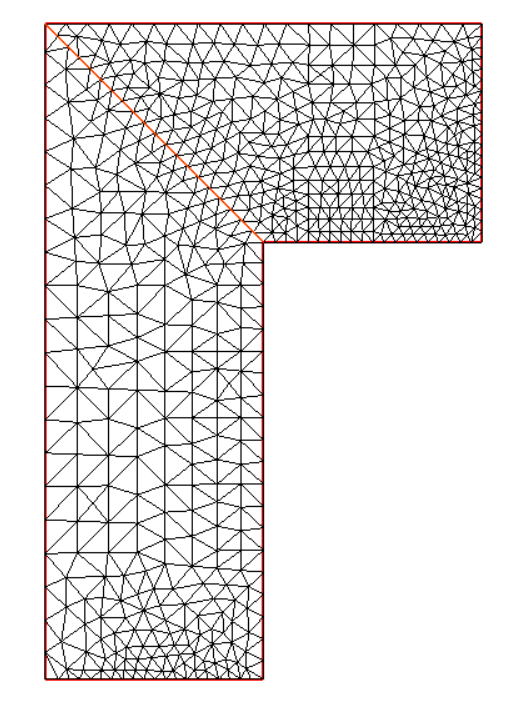
\includegraphics[width=0.7\linewidth]{mash.png}
		\caption{Сгенерированная сетка для исходной области}
	\end{figure}
	
	\begin{figure}[H]
		\centering
		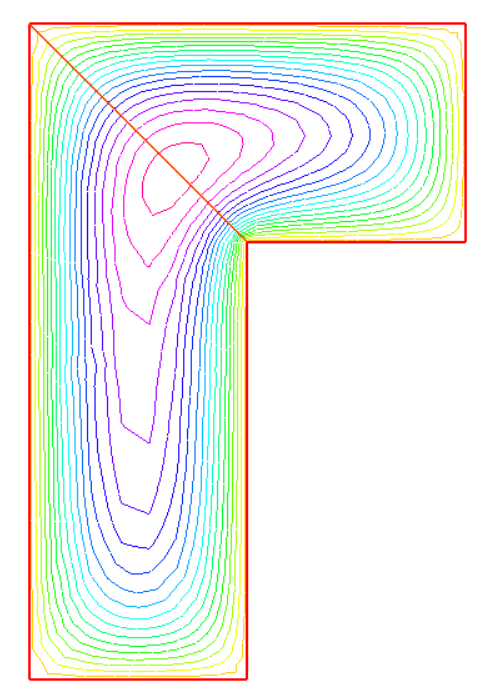
\includegraphics[width=0.7\linewidth]{solution.png}
		\caption{Решение задачи на полученной сетке}
	\end{figure}
	
	\textbf{Вывод: }\\
	
	В ходе работы мы познакомились с методом фиктивных областей для решения краевой задачи и решили упрощенную задачу на области "сапог" с помощью языка программирования FreeFem++.
	
	\end{document}